\documentclass[14pt]{extbook}
\usepackage{multicol, enumerate, enumitem, hyperref, color, soul, setspace, parskip, fancyhdr} %General Packages
\usepackage{amssymb, amsthm, amsmath, latexsym, units, mathtools} %Math Packages
\everymath{\displaystyle} %All math in Display Style
% Packages with additional options
\usepackage[headsep=0.5cm,headheight=12pt, left=1 in,right= 1 in,top= 1 in,bottom= 1 in]{geometry}
\usepackage[usenames,dvipsnames]{xcolor}
\usepackage{dashrule}  % Package to use the command below to create lines between items
\newcommand{\litem}[1]{\item#1\hspace*{-1cm}\rule{\textwidth}{0.4pt}}
\pagestyle{fancy}
\lhead{Progress Quiz 6}
\chead{}
\rhead{Version ALL}
\lfoot{4563-7456}
\cfoot{}
\rfoot{Summer C 2021}
\begin{document}

\begin{enumerate}
\litem{
Graph the equation below.\[ f(x) = -(x+2)^2 - 12 \]\begin{enumerate}[label=\Alph*.]
\begin{multicols}{2}\item 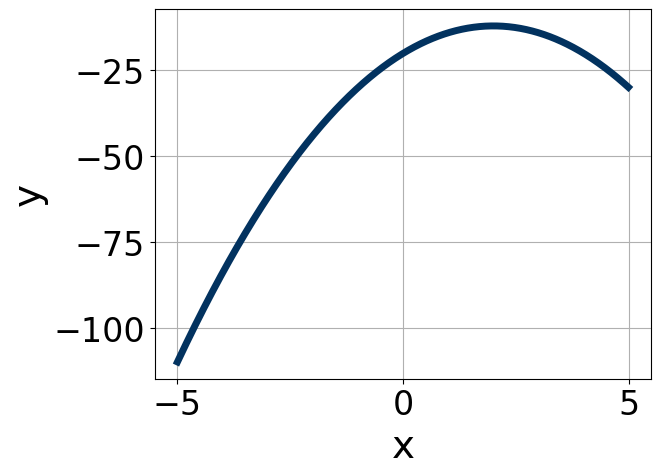
\includegraphics[width = 0.3\textwidth]{../Figures/quadraticEquationToGraphCopyAA.png}\item 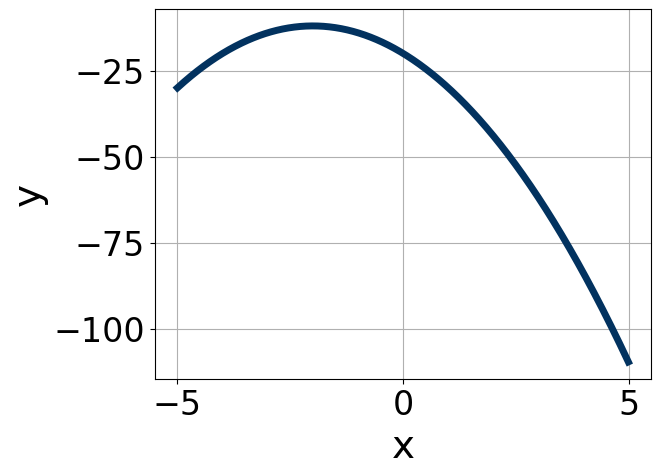
\includegraphics[width = 0.3\textwidth]{../Figures/quadraticEquationToGraphCopyBA.png}\item 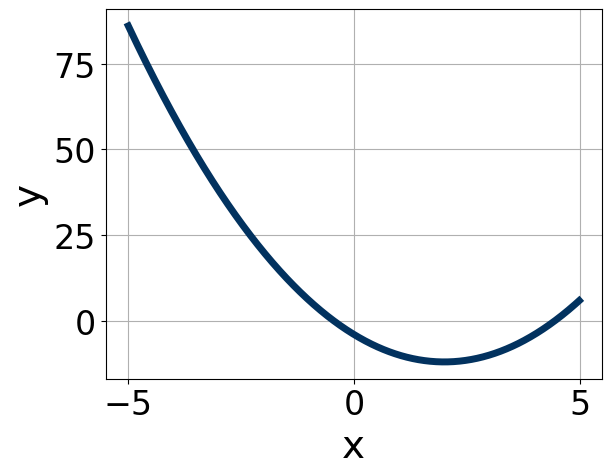
\includegraphics[width = 0.3\textwidth]{../Figures/quadraticEquationToGraphCopyCA.png}\item 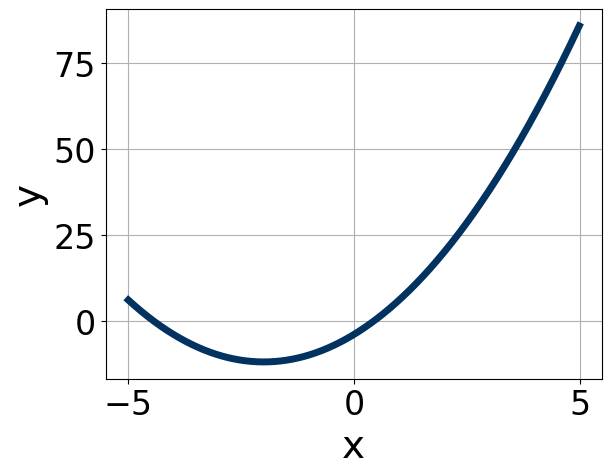
\includegraphics[width = 0.3\textwidth]{../Figures/quadraticEquationToGraphCopyDA.png}\end{multicols}\item None of the above.
\end{enumerate} }
\litem{
Factor the quadratic below. Then, choose the intervals that contain the constants in the form $(ax+b)(cx+d); b \leq d.$\[ 36x^{2} -60 x + 25 \]\begin{enumerate}[label=\Alph*.]
\item \( a \in [17.82, 18.15], \hspace*{5mm} b \in [-11, -2], \hspace*{5mm} c \in [1.94, 3.43], \text{ and } \hspace*{5mm} d \in [-5, -3] \)
\item \( a \in [-0.25, 1.19], \hspace*{5mm} b \in [-31, -21], \hspace*{5mm} c \in [0.36, 1.88], \text{ and } \hspace*{5mm} d \in [-32, -29] \)
\item \( a \in [1.53, 3.89], \hspace*{5mm} b \in [-11, -2], \hspace*{5mm} c \in [17.71, 18.48], \text{ and } \hspace*{5mm} d \in [-5, -3] \)
\item \( a \in [5.77, 6.01], \hspace*{5mm} b \in [-11, -2], \hspace*{5mm} c \in [5.38, 6.44], \text{ and } \hspace*{5mm} d \in [-5, -3] \)
\item \( \text{None of the above.} \)

\end{enumerate} }
\litem{
Factor the quadratic below. Then, choose the intervals that contain the constants in the form $(ax+b)(cx+d); b \leq d.$\[ 54x^{2} -75 x + 25 \]\begin{enumerate}[label=\Alph*.]
\item \( a \in [17.5, 20.9], \hspace*{5mm} b \in [-5, -2], \hspace*{5mm} c \in [1.7, 3.1], \text{ and } \hspace*{5mm} d \in [-5, -4] \)
\item \( a \in [8, 9.6], \hspace*{5mm} b \in [-5, -2], \hspace*{5mm} c \in [5.7, 7.9], \text{ and } \hspace*{5mm} d \in [-5, -4] \)
\item \( a \in [2.4, 4.5], \hspace*{5mm} b \in [-5, -2], \hspace*{5mm} c \in [17.2, 21.4], \text{ and } \hspace*{5mm} d \in [-5, -4] \)
\item \( a \in [0.3, 2], \hspace*{5mm} b \in [-45, -39], \hspace*{5mm} c \in [-0.1, 2.7], \text{ and } \hspace*{5mm} d \in [-32, -29] \)
\item \( \text{None of the above.} \)

\end{enumerate} }
\litem{
Graph the equation below.\[ f(x) = -(x-2)^2 - 15 \]\begin{enumerate}[label=\Alph*.]
\begin{multicols}{2}\item 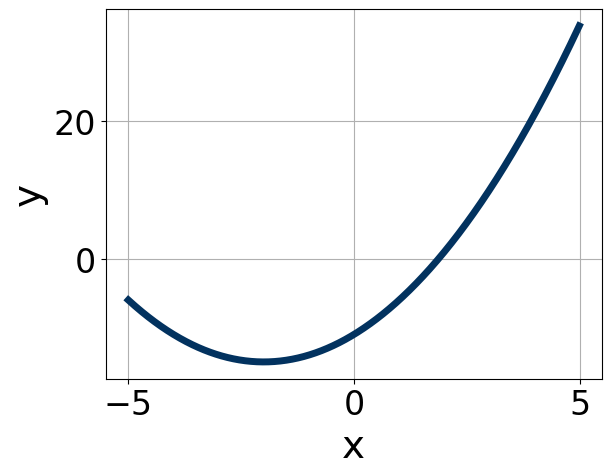
\includegraphics[width = 0.3\textwidth]{../Figures/quadraticEquationToGraphAA.png}\item 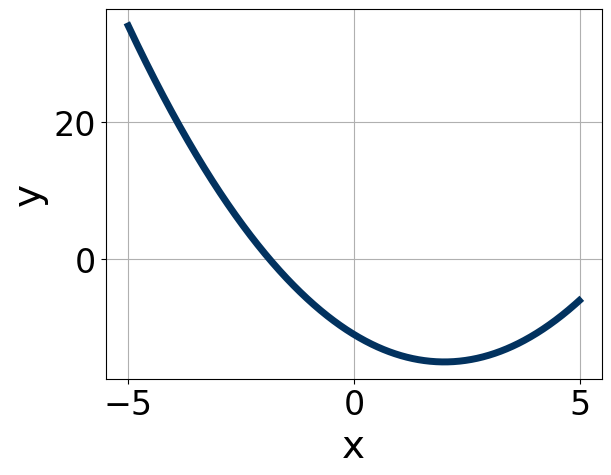
\includegraphics[width = 0.3\textwidth]{../Figures/quadraticEquationToGraphBA.png}\item 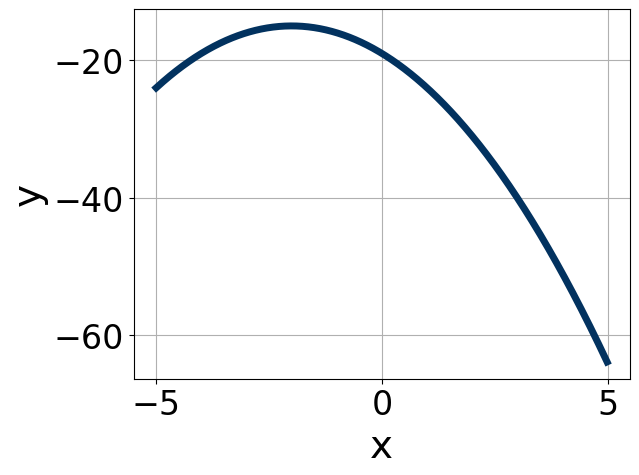
\includegraphics[width = 0.3\textwidth]{../Figures/quadraticEquationToGraphCA.png}\item 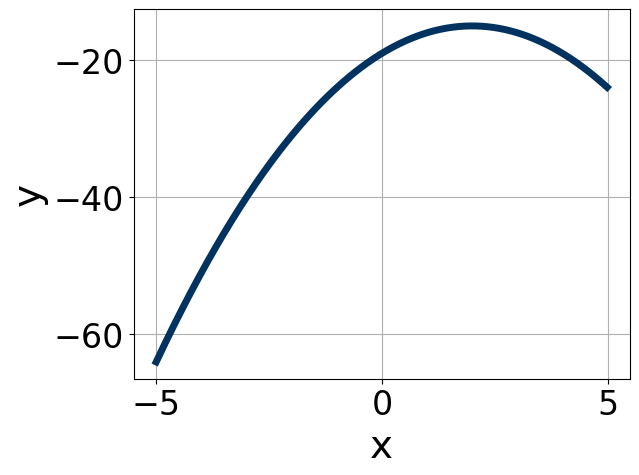
\includegraphics[width = 0.3\textwidth]{../Figures/quadraticEquationToGraphDA.png}\end{multicols}\item None of the above.
\end{enumerate} }
\litem{
Solve the quadratic equation below. Then, choose the intervals that the solutions belong to, with $x_1 \leq x_2$ (if they exist).\[ -12x^{2} -10 x + 5 = 0 \]\begin{enumerate}[label=\Alph*.]
\item \( x_1 \in [-0.5, 0.7] \text{ and } x_2 \in [0.5, 2] \)
\item \( x_1 \in [-6.2, -2.8] \text{ and } x_2 \in [12.2, 14.3] \)
\item \( x_1 \in [-1.5, -0.4] \text{ and } x_2 \in [-0.3, 1] \)
\item \( x_1 \in [-20.1, -18] \text{ and } x_2 \in [16.5, 18.7] \)
\item \( \text{There are no Real solutions.} \)

\end{enumerate} }
\litem{
Solve the quadratic equation below. Then, choose the intervals that the solutions belong to, with $x_1 \leq x_2$ (if they exist).\[ 20x^{2} -12 x -4 = 0 \]\begin{enumerate}[label=\Alph*.]
\item \( x_1 \in [-21.27, -20.75] \text{ and } x_2 \in [21.6, 22.6] \)
\item \( x_1 \in [-4.87, -4.48] \text{ and } x_2 \in [15, 18.5] \)
\item \( x_1 \in [-1.53, -0.44] \text{ and } x_2 \in [0.1, 0.4] \)
\item \( x_1 \in [-0.54, 0.22] \text{ and } x_2 \in [0.6, 2.1] \)
\item \( \text{There are no Real solutions.} \)

\end{enumerate} }
\litem{
Solve the quadratic equation below. Then, choose the intervals that the solutions $x_1$ and $x_2$ belong to, with $x_1 \leq x_2$.\[ 20x^{2} -69 x + 54 = 0 \]\begin{enumerate}[label=\Alph*.]
\item \( x_1 \in [0.71, 0.75] \text{ and } x_2 \in [3.14, 4.04] \)
\item \( x_1 \in [0.58, 0.61] \text{ and } x_2 \in [3.76, 4.87] \)
\item \( x_1 \in [23.99, 24.03] \text{ and } x_2 \in [44.08, 45.72] \)
\item \( x_1 \in [1.16, 1.22] \text{ and } x_2 \in [1.85, 2.93] \)
\item \( x_1 \in [0.45, 0.46] \text{ and } x_2 \in [5.51, 6.52] \)

\end{enumerate} }
\litem{
Solve the quadratic equation below. Then, choose the intervals that the solutions $x_1$ and $x_2$ belong to, with $x_1 \leq x_2$.\[ 15x^{2} +38 x + 24 = 0 \]\begin{enumerate}[label=\Alph*.]
\item \( x_1 \in [-2.78, -2.65] \text{ and } x_2 \in [-0.62, -0.51] \)
\item \( x_1 \in [-2.6, -1.67] \text{ and } x_2 \in [-0.74, -0.61] \)
\item \( x_1 \in [-6.56, -5.86] \text{ and } x_2 \in [-0.27, -0.26] \)
\item \( x_1 \in [-20.18, -19.34] \text{ and } x_2 \in [-18.08, -17.99] \)
\item \( x_1 \in [-1.67, -0.95] \text{ and } x_2 \in [-1.29, -1.18] \)

\end{enumerate} }
\litem{
Write the equation of the graph presented below in the form $f(x)=ax^2+bx+c$, assuming  $a=1$ or $a=-1$. Then, choose the intervals that $a, b,$ and $c$ belong to.
\begin{center}
    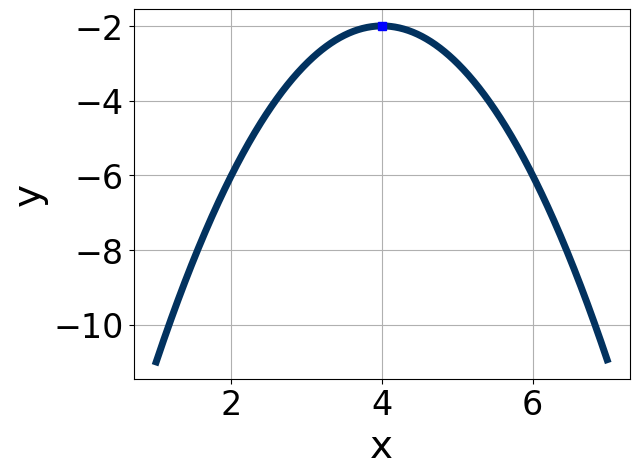
\includegraphics[width=0.5\textwidth]{../Figures/quadraticGraphToEquationA.png}
\end{center}
\begin{enumerate}[label=\Alph*.]
\item \( a \in [-1.6, -0.8], \hspace*{5mm} b \in [7, 13], \text{ and } \hspace*{5mm} c \in [-19, -17] \)
\item \( a \in [-1.6, -0.8], \hspace*{5mm} b \in [-8, -5], \text{ and } \hspace*{5mm} c \in [-15, -11] \)
\item \( a \in [-1.6, -0.8], \hspace*{5mm} b \in [-8, -5], \text{ and } \hspace*{5mm} c \in [-19, -17] \)
\item \( a \in [-0.2, 1.6], \hspace*{5mm} b \in [7, 13], \text{ and } \hspace*{5mm} c \in [13, 18] \)
\item \( a \in [-0.2, 1.6], \hspace*{5mm} b \in [-8, -5], \text{ and } \hspace*{5mm} c \in [13, 18] \)

\end{enumerate} }
\litem{
Write the equation of the graph presented below in the form $f(x)=ax^2+bx+c$, assuming  $a=1$ or $a=-1$. Then, choose the intervals that $a, b,$ and $c$ belong to.
\begin{center}
    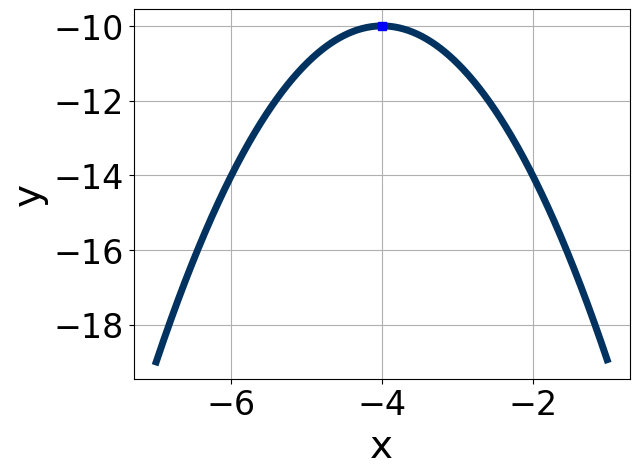
\includegraphics[width=0.5\textwidth]{../Figures/quadraticGraphToEquationCopyA.png}
\end{center}
\begin{enumerate}[label=\Alph*.]
\item \( a \in [1, 3], \hspace*{5mm} b \in [-10, -7], \text{ and } \hspace*{5mm} c \in [5, 9] \)
\item \( a \in [1, 3], \hspace*{5mm} b \in [6, 12], \text{ and } \hspace*{5mm} c \in [5, 9] \)
\item \( a \in [-3, 0], \hspace*{5mm} b \in [6, 12], \text{ and } \hspace*{5mm} c \in [-7, -1] \)
\item \( a \in [-3, 0], \hspace*{5mm} b \in [6, 12], \text{ and } \hspace*{5mm} c \in [-26, -23] \)
\item \( a \in [-3, 0], \hspace*{5mm} b \in [-10, -7], \text{ and } \hspace*{5mm} c \in [-26, -23] \)

\end{enumerate} }
\litem{
Graph the equation below.\[ f(x) = (x+1)^2 - 10 \]\begin{enumerate}[label=\Alph*.]
\begin{multicols}{2}\item 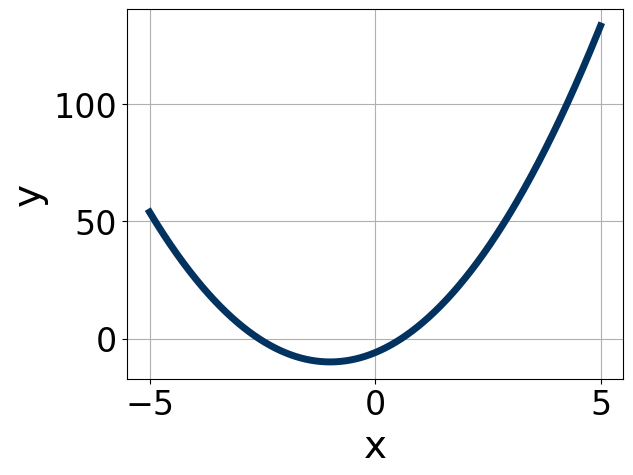
\includegraphics[width = 0.3\textwidth]{../Figures/quadraticEquationToGraphCopyAB.png}\item 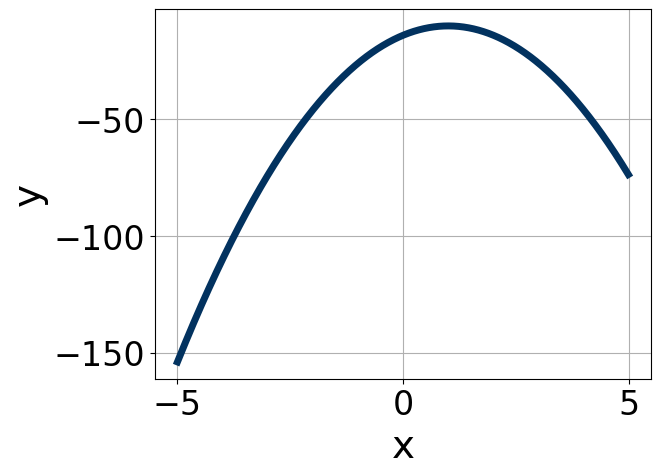
\includegraphics[width = 0.3\textwidth]{../Figures/quadraticEquationToGraphCopyBB.png}\item 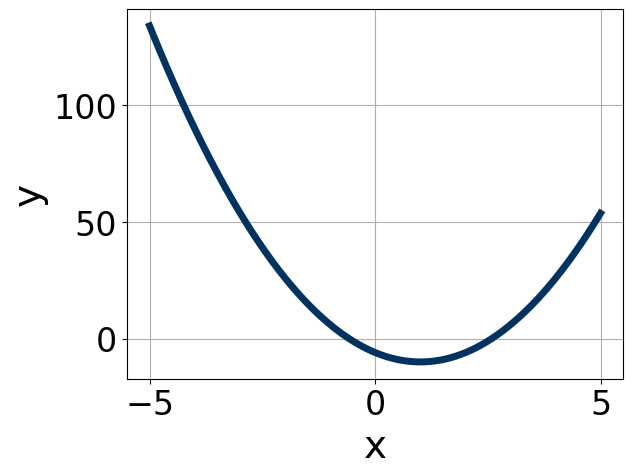
\includegraphics[width = 0.3\textwidth]{../Figures/quadraticEquationToGraphCopyCB.png}\item 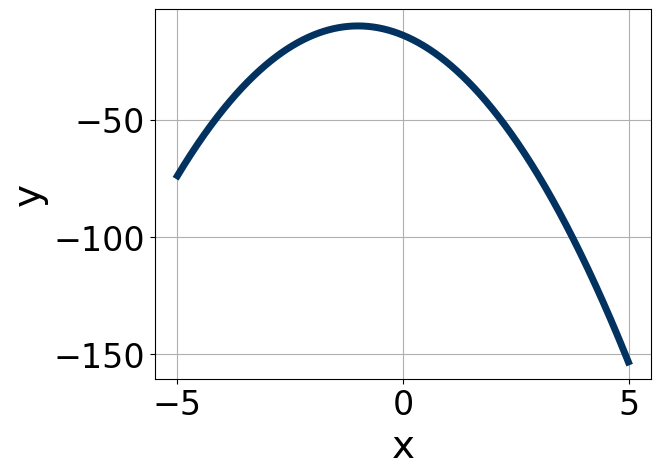
\includegraphics[width = 0.3\textwidth]{../Figures/quadraticEquationToGraphCopyDB.png}\end{multicols}\item None of the above.
\end{enumerate} }
\litem{
Factor the quadratic below. Then, choose the intervals that contain the constants in the form $(ax+b)(cx+d); b \leq d.$\[ 36x^{2} +60 x + 25 \]\begin{enumerate}[label=\Alph*.]
\item \( a \in [5.5, 6.7], \hspace*{5mm} b \in [4, 10], \hspace*{5mm} c \in [4.4, 7.1], \text{ and } \hspace*{5mm} d \in [5, 10] \)
\item \( a \in [-1.8, 1.6], \hspace*{5mm} b \in [28, 34], \hspace*{5mm} c \in [0.7, 2.5], \text{ and } \hspace*{5mm} d \in [28, 31] \)
\item \( a \in [10.3, 14.2], \hspace*{5mm} b \in [4, 10], \hspace*{5mm} c \in [1.1, 4.7], \text{ and } \hspace*{5mm} d \in [5, 10] \)
\item \( a \in [1.1, 4.1], \hspace*{5mm} b \in [4, 10], \hspace*{5mm} c \in [11.7, 12.4], \text{ and } \hspace*{5mm} d \in [5, 10] \)
\item \( \text{None of the above.} \)

\end{enumerate} }
\litem{
Factor the quadratic below. Then, choose the intervals that contain the constants in the form $(ax+b)(cx+d); b \leq d.$\[ 24x^{2} +50 x + 25 \]\begin{enumerate}[label=\Alph*.]
\item \( a \in [-0.9, 2.5], \hspace*{5mm} b \in [16, 22], \hspace*{5mm} c \in [0.8, 1.14], \text{ and } \hspace*{5mm} d \in [30, 34] \)
\item \( a \in [5.3, 8.8], \hspace*{5mm} b \in [5, 11], \hspace*{5mm} c \in [3.86, 4.62], \text{ and } \hspace*{5mm} d \in [4, 9] \)
\item \( a \in [9.4, 14.1], \hspace*{5mm} b \in [5, 11], \hspace*{5mm} c \in [1.84, 2.09], \text{ and } \hspace*{5mm} d \in [4, 9] \)
\item \( a \in [2.9, 3.4], \hspace*{5mm} b \in [5, 11], \hspace*{5mm} c \in [4.77, 8.57], \text{ and } \hspace*{5mm} d \in [4, 9] \)
\item \( \text{None of the above.} \)

\end{enumerate} }
\litem{
Graph the equation below.\[ f(x) = -(x-2)^2 + 10 \]\begin{enumerate}[label=\Alph*.]
\begin{multicols}{2}\item 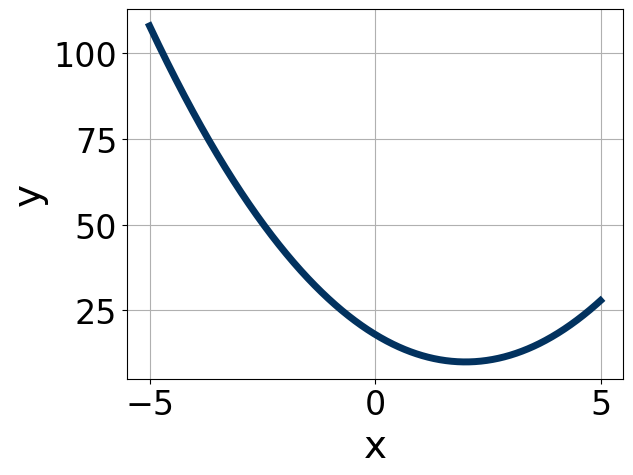
\includegraphics[width = 0.3\textwidth]{../Figures/quadraticEquationToGraphAB.png}\item 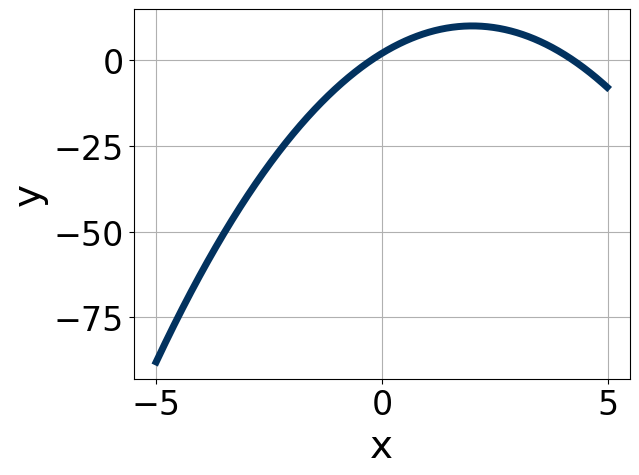
\includegraphics[width = 0.3\textwidth]{../Figures/quadraticEquationToGraphBB.png}\item 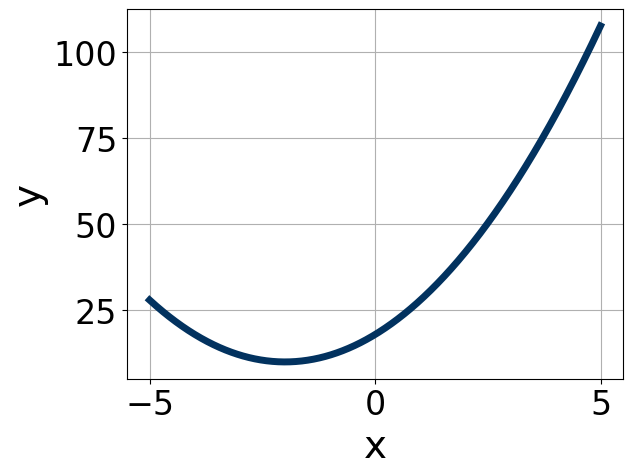
\includegraphics[width = 0.3\textwidth]{../Figures/quadraticEquationToGraphCB.png}\item 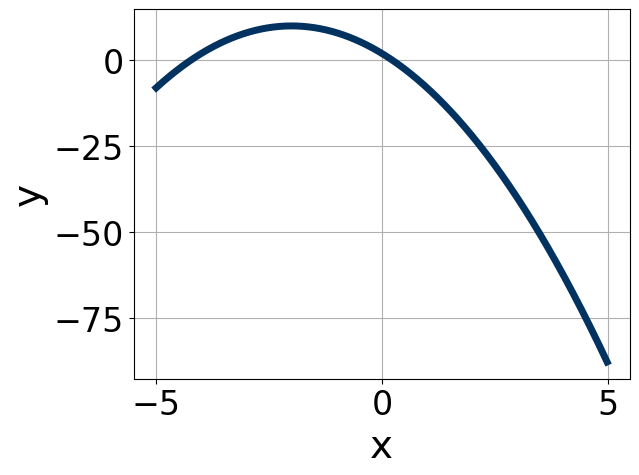
\includegraphics[width = 0.3\textwidth]{../Figures/quadraticEquationToGraphDB.png}\end{multicols}\item None of the above.
\end{enumerate} }
\litem{
Solve the quadratic equation below. Then, choose the intervals that the solutions belong to, with $x_1 \leq x_2$ (if they exist).\[ -15x^{2} +14 x + 4 = 0 \]\begin{enumerate}[label=\Alph*.]
\item \( x_1 \in [-18.23, -17.35] \text{ and } x_2 \in [2.3, 5.3] \)
\item \( x_1 \in [-20.79, -19.67] \text{ and } x_2 \in [20.9, 21.4] \)
\item \( x_1 \in [-0.95, -0.13] \text{ and } x_2 \in [0.9, 1.9] \)
\item \( x_1 \in [-1.63, -0.76] \text{ and } x_2 \in [-0.8, 1] \)
\item \( \text{There are no Real solutions.} \)

\end{enumerate} }
\litem{
Solve the quadratic equation below. Then, choose the intervals that the solutions belong to, with $x_1 \leq x_2$ (if they exist).\[ 20x^{2} -12 x -4 = 0 \]\begin{enumerate}[label=\Alph*.]
\item \( x_1 \in [-2.8, -0.6] \text{ and } x_2 \in [-0.14, 0.51] \)
\item \( x_1 \in [-6.1, -3.5] \text{ and } x_2 \in [16.46, 17.17] \)
\item \( x_1 \in [-22.6, -21] \text{ and } x_2 \in [21, 22.99] \)
\item \( x_1 \in [-0.8, 0.1] \text{ and } x_2 \in [0.73, 0.88] \)
\item \( \text{There are no Real solutions.} \)

\end{enumerate} }
\litem{
Solve the quadratic equation below. Then, choose the intervals that the solutions $x_1$ and $x_2$ belong to, with $x_1 \leq x_2$.\[ 10x^{2} -53 x + 36 = 0 \]\begin{enumerate}[label=\Alph*.]
\item \( x_1 \in [0.32, 0.5] \text{ and } x_2 \in [8.64, 9.16] \)
\item \( x_1 \in [7.96, 8.19] \text{ and } x_2 \in [44.81, 45.46] \)
\item \( x_1 \in [0.71, 0.83] \text{ and } x_2 \in [4.25, 5.03] \)
\item \( x_1 \in [0.81, 0.92] \text{ and } x_2 \in [3.77, 4.23] \)
\item \( x_1 \in [1.5, 1.82] \text{ and } x_2 \in [1.57, 3] \)

\end{enumerate} }
\litem{
Solve the quadratic equation below. Then, choose the intervals that the solutions $x_1$ and $x_2$ belong to, with $x_1 \leq x_2$.\[ 15x^{2} +38 x + 24 = 0 \]\begin{enumerate}[label=\Alph*.]
\item \( x_1 \in [-2.19, 0.62] \text{ and } x_2 \in [-1.26, -1.2] \)
\item \( x_1 \in [-3.17, -1.5] \text{ and } x_2 \in [-0.82, -0.45] \)
\item \( x_1 \in [-5.27, -3.33] \text{ and } x_2 \in [-0.41, -0.32] \)
\item \( x_1 \in [-6.8, -5.15] \text{ and } x_2 \in [-0.33, -0.24] \)
\item \( x_1 \in [-20.47, -19.44] \text{ and } x_2 \in [-18.02, -17.91] \)

\end{enumerate} }
\litem{
Write the equation of the graph presented below in the form $f(x)=ax^2+bx+c$, assuming  $a=1$ or $a=-1$. Then, choose the intervals that $a, b,$ and $c$ belong to.
\begin{center}
    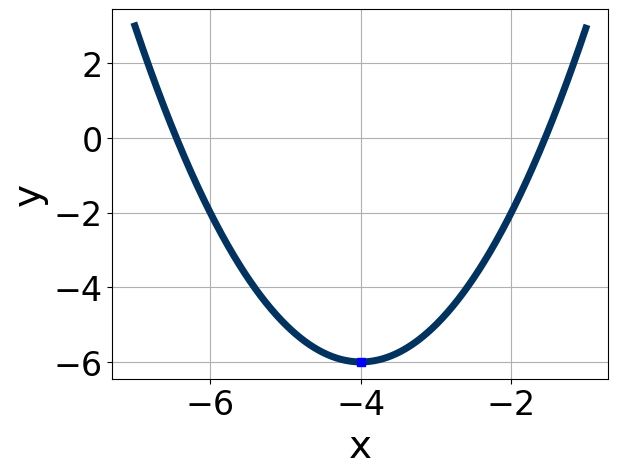
\includegraphics[width=0.5\textwidth]{../Figures/quadraticGraphToEquationB.png}
\end{center}
\begin{enumerate}[label=\Alph*.]
\item \( a \in [1, 2], \hspace*{5mm} b \in [6, 13], \text{ and } \hspace*{5mm} c \in [8, 11] \)
\item \( a \in [-3, 0], \hspace*{5mm} b \in [6, 13], \text{ and } \hspace*{5mm} c \in [-25, -19] \)
\item \( a \in [-3, 0], \hspace*{5mm} b \in [-10, -6], \text{ and } \hspace*{5mm} c \in [-25, -19] \)
\item \( a \in [1, 2], \hspace*{5mm} b \in [-10, -6], \text{ and } \hspace*{5mm} c \in [22, 26] \)
\item \( a \in [1, 2], \hspace*{5mm} b \in [-10, -6], \text{ and } \hspace*{5mm} c \in [8, 11] \)

\end{enumerate} }
\litem{
Write the equation of the graph presented below in the form $f(x)=ax^2+bx+c$, assuming  $a=1$ or $a=-1$. Then, choose the intervals that $a, b,$ and $c$ belong to.
\begin{center}
    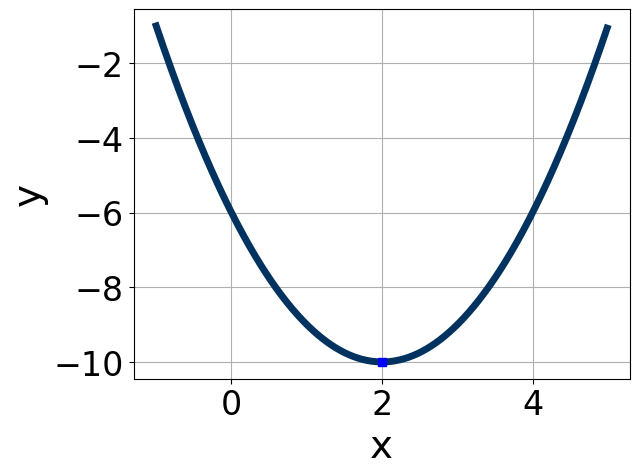
\includegraphics[width=0.5\textwidth]{../Figures/quadraticGraphToEquationCopyB.png}
\end{center}
\begin{enumerate}[label=\Alph*.]
\item \( a \in [-0.9, 1.7], \hspace*{5mm} b \in [-4, 0], \text{ and } \hspace*{5mm} c \in [-9, -4] \)
\item \( a \in [-1.7, 0.1], \hspace*{5mm} b \in [-4, 0], \text{ and } \hspace*{5mm} c \in [-14, -12] \)
\item \( a \in [-1.7, 0.1], \hspace*{5mm} b \in [3, 6], \text{ and } \hspace*{5mm} c \in [-14, -12] \)
\item \( a \in [-0.9, 1.7], \hspace*{5mm} b \in [3, 6], \text{ and } \hspace*{5mm} c \in [-9, -4] \)
\item \( a \in [-0.9, 1.7], \hspace*{5mm} b \in [3, 6], \text{ and } \hspace*{5mm} c \in [13, 15] \)

\end{enumerate} }
\litem{
Graph the equation below.\[ f(x) = -(x+2)^2 - 16 \]\begin{enumerate}[label=\Alph*.]
\begin{multicols}{2}\item 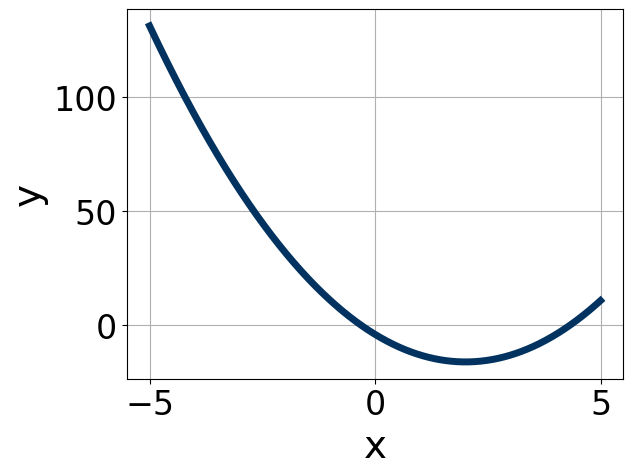
\includegraphics[width = 0.3\textwidth]{../Figures/quadraticEquationToGraphCopyAC.png}\item 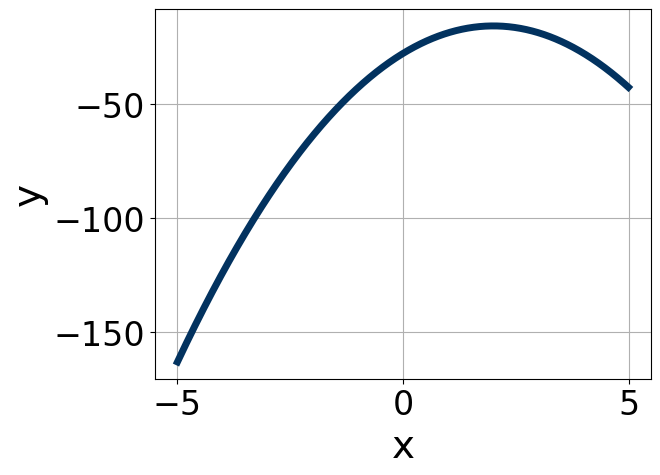
\includegraphics[width = 0.3\textwidth]{../Figures/quadraticEquationToGraphCopyBC.png}\item 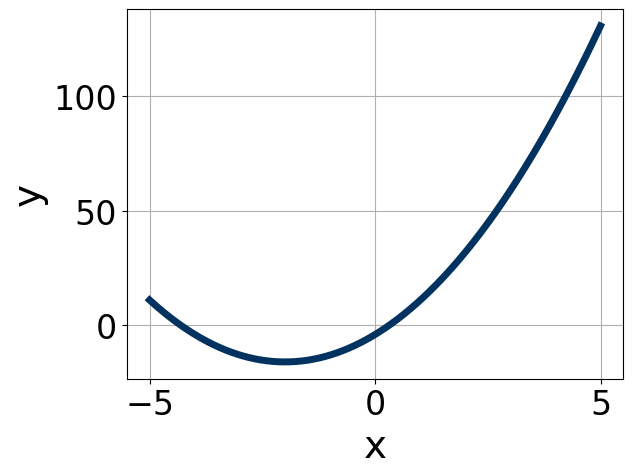
\includegraphics[width = 0.3\textwidth]{../Figures/quadraticEquationToGraphCopyCC.png}\item 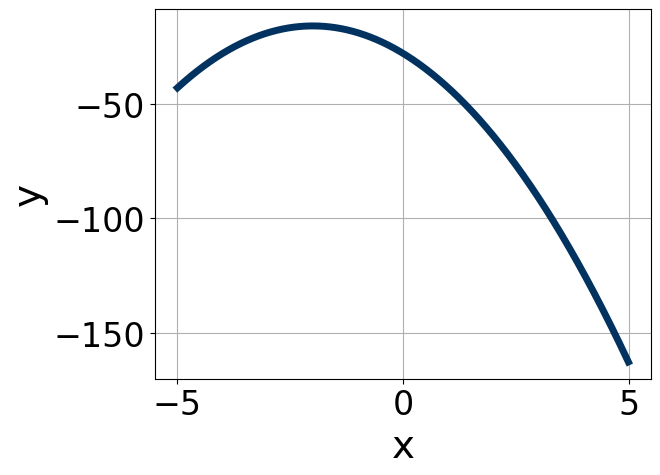
\includegraphics[width = 0.3\textwidth]{../Figures/quadraticEquationToGraphCopyDC.png}\end{multicols}\item None of the above.
\end{enumerate} }
\litem{
Factor the quadratic below. Then, choose the intervals that contain the constants in the form $(ax+b)(cx+d); b \leq d.$\[ 36x^{2} +61 x + 20 \]\begin{enumerate}[label=\Alph*.]
\item \( a \in [7, 14], \hspace*{5mm} b \in [4, 5], \hspace*{5mm} c \in [3.26, 4.33], \text{ and } \hspace*{5mm} d \in [3, 9] \)
\item \( a \in [-3, 2], \hspace*{5mm} b \in [15, 19], \hspace*{5mm} c \in [-0.27, 1.45], \text{ and } \hspace*{5mm} d \in [41, 52] \)
\item \( a \in [3, 8], \hspace*{5mm} b \in [4, 5], \hspace*{5mm} c \in [7.89, 8.53], \text{ and } \hspace*{5mm} d \in [3, 9] \)
\item \( a \in [27, 29], \hspace*{5mm} b \in [4, 5], \hspace*{5mm} c \in [-0.27, 1.45], \text{ and } \hspace*{5mm} d \in [3, 9] \)
\item \( \text{None of the above.} \)

\end{enumerate} }
\litem{
Factor the quadratic below. Then, choose the intervals that contain the constants in the form $(ax+b)(cx+d); b \leq d.$\[ 24x^{2} -10 x -25 \]\begin{enumerate}[label=\Alph*.]
\item \( a \in [7.89, 8.65], \hspace*{5mm} b \in [-8, -4], \hspace*{5mm} c \in [1.8, 4.8], \text{ and } \hspace*{5mm} d \in [1, 6] \)
\item \( a \in [-1.13, 1.53], \hspace*{5mm} b \in [-30, -28], \hspace*{5mm} c \in [0.5, 1.7], \text{ and } \hspace*{5mm} d \in [19, 23] \)
\item \( a \in [2.93, 4.07], \hspace*{5mm} b \in [-8, -4], \hspace*{5mm} c \in [4.8, 8.9], \text{ and } \hspace*{5mm} d \in [1, 6] \)
\item \( a \in [1.83, 3.68], \hspace*{5mm} b \in [-8, -4], \hspace*{5mm} c \in [11.5, 14.6], \text{ and } \hspace*{5mm} d \in [1, 6] \)
\item \( \text{None of the above.} \)

\end{enumerate} }
\litem{
Graph the equation below.\[ f(x) = (x+1)^2 - 17 \]\begin{enumerate}[label=\Alph*.]
\begin{multicols}{2}\item 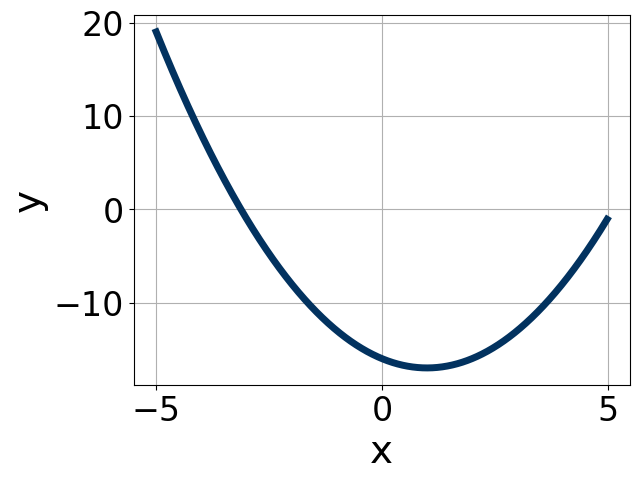
\includegraphics[width = 0.3\textwidth]{../Figures/quadraticEquationToGraphAC.png}\item 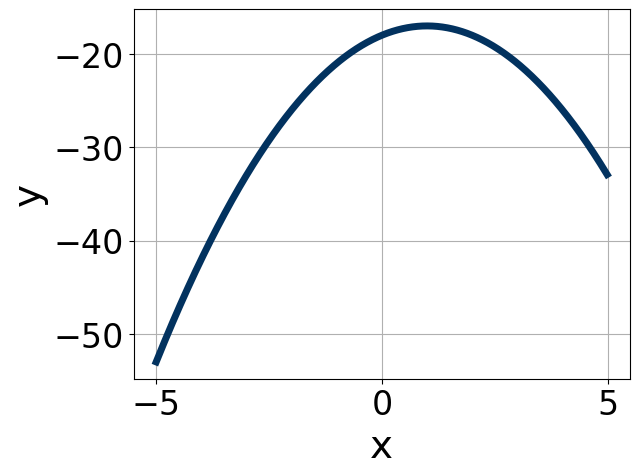
\includegraphics[width = 0.3\textwidth]{../Figures/quadraticEquationToGraphBC.png}\item 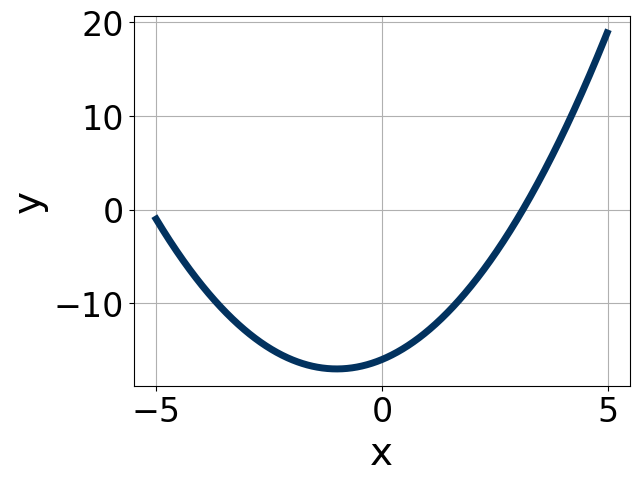
\includegraphics[width = 0.3\textwidth]{../Figures/quadraticEquationToGraphCC.png}\item 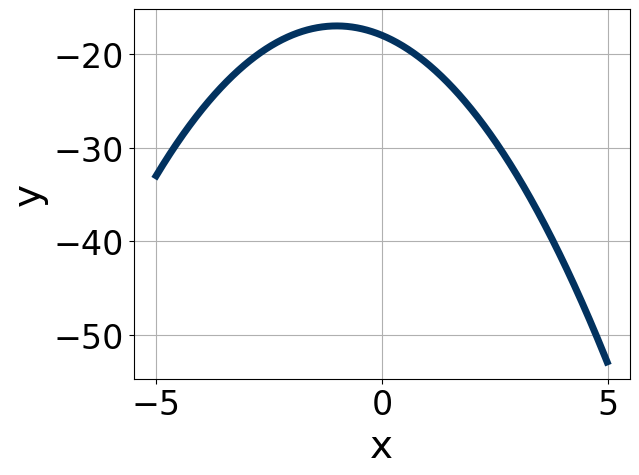
\includegraphics[width = 0.3\textwidth]{../Figures/quadraticEquationToGraphDC.png}\end{multicols}\item None of the above.
\end{enumerate} }
\litem{
Solve the quadratic equation below. Then, choose the intervals that the solutions belong to, with $x_1 \leq x_2$ (if they exist).\[ 14x^{2} -11 x -8 = 0 \]\begin{enumerate}[label=\Alph*.]
\item \( x_1 \in [-7.7, -6.2] \text{ and } x_2 \in [16.4, 19.3] \)
\item \( x_1 \in [-1.5, -1.1] \text{ and } x_2 \in [-1.2, 1.1] \)
\item \( x_1 \in [-0.9, -0.3] \text{ and } x_2 \in [0.8, 2.2] \)
\item \( x_1 \in [-24, -22.8] \text{ and } x_2 \in [24, 24.8] \)
\item \( \text{There are no Real solutions.} \)

\end{enumerate} }
\litem{
Solve the quadratic equation below. Then, choose the intervals that the solutions belong to, with $x_1 \leq x_2$ (if they exist).\[ 16x^{2} -11 x -4 = 0 \]\begin{enumerate}[label=\Alph*.]
\item \( x_1 \in [-20, -17.4] \text{ and } x_2 \in [18.69, 19.94] \)
\item \( x_1 \in [-4.9, -3.6] \text{ and } x_2 \in [14.49, 15.55] \)
\item \( x_1 \in [-2.4, -0.6] \text{ and } x_2 \in [0.04, 0.59] \)
\item \( x_1 \in [-0.8, 2.1] \text{ and } x_2 \in [0.65, 1.04] \)
\item \( \text{There are no Real solutions.} \)

\end{enumerate} }
\litem{
Solve the quadratic equation below. Then, choose the intervals that the solutions $x_1$ and $x_2$ belong to, with $x_1 \leq x_2$.\[ 25x^{2} -60 x + 36 = 0 \]\begin{enumerate}[label=\Alph*.]
\item \( x_1 \in [0.29, 0.54] \text{ and } x_2 \in [3.38, 4.56] \)
\item \( x_1 \in [1.08, 1.81] \text{ and } x_2 \in [0.27, 1.73] \)
\item \( x_1 \in [0.51, 0.78] \text{ and } x_2 \in [1.98, 3.55] \)
\item \( x_1 \in [0.21, 0.38] \text{ and } x_2 \in [5.11, 7.21] \)
\item \( x_1 \in [29.71, 30.02] \text{ and } x_2 \in [29.92, 30.47] \)

\end{enumerate} }
\litem{
Solve the quadratic equation below. Then, choose the intervals that the solutions $x_1$ and $x_2$ belong to, with $x_1 \leq x_2$.\[ 25x^{2} -65 x + 36 = 0 \]\begin{enumerate}[label=\Alph*.]
\item \( x_1 \in [0.51, 0.61] \text{ and } x_2 \in [1.82, 3.36] \)
\item \( x_1 \in [0.78, 0.86] \text{ and } x_2 \in [1.62, 2.15] \)
\item \( x_1 \in [0.39, 0.46] \text{ and } x_2 \in [2.81, 3.66] \)
\item \( x_1 \in [19.95, 20.11] \text{ and } x_2 \in [44.95, 45.23] \)
\item \( x_1 \in [0.33, 0.37] \text{ and } x_2 \in [3.73, 4.59] \)

\end{enumerate} }
\litem{
Write the equation of the graph presented below in the form $f(x)=ax^2+bx+c$, assuming  $a=1$ or $a=-1$. Then, choose the intervals that $a, b,$ and $c$ belong to.
\begin{center}
    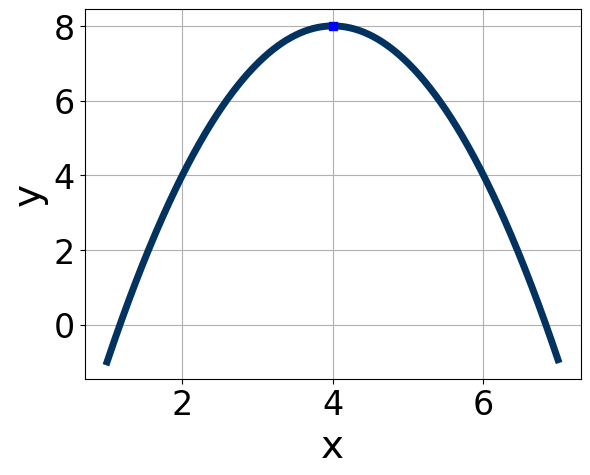
\includegraphics[width=0.5\textwidth]{../Figures/quadraticGraphToEquationC.png}
\end{center}
\begin{enumerate}[label=\Alph*.]
\item \( a \in [-2, 0], \hspace*{5mm} b \in [-12, -7], \text{ and } \hspace*{5mm} c \in [-26, -22] \)
\item \( a \in [0, 4], \hspace*{5mm} b \in [-12, -7], \text{ and } \hspace*{5mm} c \in [24, 25] \)
\item \( a \in [-2, 0], \hspace*{5mm} b \in [7, 9], \text{ and } \hspace*{5mm} c \in [-9, -6] \)
\item \( a \in [0, 4], \hspace*{5mm} b \in [7, 9], \text{ and } \hspace*{5mm} c \in [24, 25] \)
\item \( a \in [-2, 0], \hspace*{5mm} b \in [-12, -7], \text{ and } \hspace*{5mm} c \in [-9, -6] \)

\end{enumerate} }
\litem{
Write the equation of the graph presented below in the form $f(x)=ax^2+bx+c$, assuming  $a=1$ or $a=-1$. Then, choose the intervals that $a, b,$ and $c$ belong to.
\begin{center}
    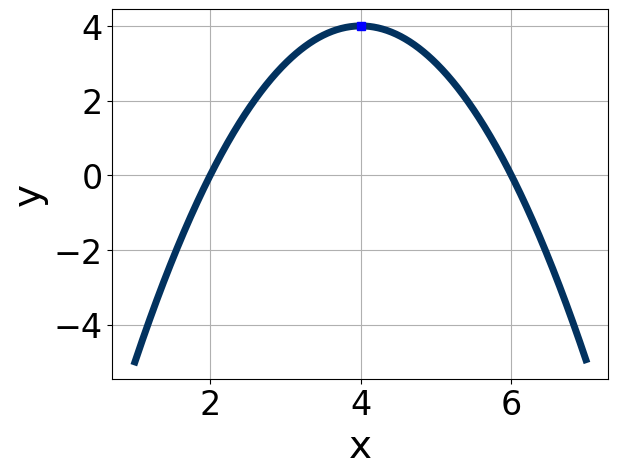
\includegraphics[width=0.5\textwidth]{../Figures/quadraticGraphToEquationCopyC.png}
\end{center}
\begin{enumerate}[label=\Alph*.]
\item \( a \in [-1.6, -0.7], \hspace*{5mm} b \in [5, 11], \text{ and } \hspace*{5mm} c \in [-15, -11] \)
\item \( a \in [-1.6, -0.7], \hspace*{5mm} b \in [-8, -7], \text{ and } \hspace*{5mm} c \in [-15, -11] \)
\item \( a \in [0.3, 2], \hspace*{5mm} b \in [5, 11], \text{ and } \hspace*{5mm} c \in [18, 21] \)
\item \( a \in [-1.6, -0.7], \hspace*{5mm} b \in [-8, -7], \text{ and } \hspace*{5mm} c \in [-22, -19] \)
\item \( a \in [0.3, 2], \hspace*{5mm} b \in [-8, -7], \text{ and } \hspace*{5mm} c \in [18, 21] \)

\end{enumerate} }
\end{enumerate}

\end{document}